%%%%%%%%%%%%%%%%%%%%%%%%%%%%%%%%%%%%%%%%%%%%%%%%%%%%%%%%%%%%%%%%%%%%%%%%%%%%%%%%%%%%%
% Template revision history:
% BS02022: Revised by Sukumar Natarajan, s.natarajan@bath.ac.uk
% BS2021: Revised by Filip Jorissen, filip.jorissen@kuleuven.be
% BS2019: Revised by Alessandro Prada, alessandro.prada@unitn.it
% BS2017: Initial version by Michael Wetter, mwetter@lbl.gov
%%%%%%%%%%%%%%%%%%%%%%%%%%%%%%%%%%%%%%%%%%%%%%%%%%%%%%%%%%%%%%%%%%%%%%%%%%%%%%%%%%%%%

\documentclass[twocolumn, a4paper,10pt]{article}
\usepackage[top=2.5cm, bottom=2.5cm, left=2.0cm, right=2.0cm,
columnsep=0.8cm]{geometry}
\usepackage{enumitem}
\usepackage[hyphens]{url}
\usepackage[colorlinks,allcolors=blue]{hyperref}
\usepackage{boxedminipage}
\usepackage{nopageno}
\usepackage{graphicx}
\usepackage{amsmath}
\usepackage{natbib}
\usepackage[font=it]{caption}
\usepackage[usenames,dvipsnames]{xcolor}
\usepackage{listings}
\usepackage{caption}
\usepackage{subcaption}
\usepackage{bookmark}
\usepackage{float}
\DeclareCaptionType[within=section]{mat}[Matrix]


%-----------------------------SET SKIP SPACES -------------------------------------------------------------------
\setlength{\abovecaptionskip}{0pt}
\setlength{\belowcaptionskip}{3pt}
\setlength{\parindent}{0pt}
\setlength{\parskip}{3pt}
%\renewcommand{\baselinestretch}{0.7}
% FOR enumerates
\setlist{itemsep=-0.1cm,topsep=0.1cm,labelsep=0.3cm}
\setenumerate{leftmargin=*}
\setcounter{secnumdepth}{-1}
%-----------------------------SET FONTS -------------------------------------------------------------------
% Set fonts for title, section and subsection headings
\makeatletter
\renewcommand\title[1]{\gdef\@title{\fontsize{12pt}{2pt}\bfseries{#1}}}
\makeatletter
\renewcommand\section{\@startsection{section}{1}{\z@}{3pt}{3pt}{\normalfont\large\bfseries}}
% \normalfont\large
\makeatletter
\renewcommand\subsection{\@startsection{subsection}{1}{\z@}{\z@}{\z@}{\normalfont\normalsize\bfseries}}
\makeatletter
\renewcommand\subsection{\@startsection{subsection}{1}{\z@}{\z@}{0.1pt}{\normalfont\normalsize\bfseries}}
\renewcommand\refname{References}
%END OF THE SETUP
%%%%%%%%%%%%%%%%%%%%%%%%%%%%%%%%%%%%%%%%%%%%%%%%%%%%%%%%%%%%

%%%%%%%%%%%%%%%%%%%%%%%%   TITLE   %%%%%%%%%%%%%%%%%%%%%%%%%%%%%%%
%%% Please keep the \vspace{4pt} at the top
\title{%
Project Report for: Neapolitan Card Classifier\\																								% Line 1
%%% Please keep the \vspace{4pt} between lines in the title
\vspace{4pt}
Real world cases and Humanitarian implications \[LM-32 a.a. 2023/2024\]
} 																																% Line 2 
%If there is no second line then just put \phantom{Line 2} here
%%% Change or delete text before "\\" on the lines below to keep the layout but don't remove the "\\"
%%% Do not exceed more than 6 lines for authors and affiliations
\author{																																														% Line 3
Emmanuele Virginio Coppola$^1$\\ 																										% Line 4
$^1$ emmanuele.coppola@studenti.unitn.it\\ 																																	% Line 5
% comment the lines below and add \phantom{} lines as needed to reach a total of 10 lines
%\textit{(The names and affiliations SHOULD NOT be included in the draft submitted for review)}\\ 			 			  	% Line 7
%\textit{(leave blank up to line 10 - remove line numbering from final version)}\\ 															% Line 8
\phantom{Line 9}} 																																									% Line 9
\date{\vspace{-0.5cm}}	% remove default date and replace the Blank 10th line														% Line 10
%END OF THE TITLE
%%%%%%%%%%%%%%%%%%%%%%%%%%%%%%%%%%%%%%%%%%%%%%%%%%%%%%%%%%%%
\begin{document}

\maketitle
\begin{figure}
  \centering


\includegraphics[scale=0.6]{img/Logo.pdf}
\end{figure}
\section*{Abstract}	% Section headings need to be upper and lower case.
\addtocounter{section}{1}

This paper proposes a novel approach for playing card identification applying computer vision technics on images of the cards. The process begins with capturing a 24-bit true-color image of the card using a mobile phone. Subsequently, the image undergoes several preprocessing steps: downsampling, conversion to a 256-grayscale format, and binary conversion for the recognition task.

The main stages of processing involve identifying the card shape through contour approximation, determining the four angles of the card, and rectifying the perspective to align the card vertically. Once the card shape is accurately approximated, and projected a contour shape matching technique is applied using the Hu invariant moment, which is robust against rotation, ensuring reliable identification.

Furthermore, a classifier is employed to determine both the value and suit of the card. By integrating these techniques, visually impaired individuals can participate in Italian card games like scopa or other games with different card decks. This enables these people to experience the enjoyment and social interaction associated with card games.

\section*{Introduction}
In recent years, the intersection of computer vision and assistive technology has witnessed remarkable advancements, particularly in enhancing accessibility and inclusivity for individuals with visual impairments. Among various applications, the recognition of playing cards stands as a notable example with potential implications for facilitating leisure activities and social engagement. Traditional card games, deeply ingrained in cultural and social contexts, often pose challenges for visually impaired individuals due to their reliance on visual cues for gameplay. Even if there exist card games that use special textures or braille in the card, not every card deck have this systems in place.

This paper introduces a novel approach to playing card recognition, leveraging the intrinsic features of card faces as identification targets. Unlike conventional methods that primarily focus on text or pattern recognition, our proposed methodology centers on the unique visual characteristics of playing cards, enabling robust and efficient identification. By harnessing the capabilities of modern mobile devices, particularly their imaging capabilities, we aim to bridge the accessibility gap and empower visually impaired individuals to partake in card-based leisure activities.

The methodology outlined in this paper encompasses a series of processing steps, including image preprocessing, contour approximation, perspective rectification, and classification. Notably, the utilization of the Hu invariant moment for contour shape matching ensures rotation invariance, thus enabling accurate card recognition regardless of orientation not only of the card, but even the figures in them. Furthermore, the integration of a classifier facilitates the identification of both card value and suit, enhancing the utility and versatility of the proposed system.

Beyond its technical merits, the significance of playing card recognition extends to its potential societal impact, particularly in the realm of accessibility and inclusion. By enabling visually impaired individuals to participate in card games, such as traditional Italian games like scopa, our approach fosters social interaction, cognitive stimulation, and recreational enjoyment.

\subsection*{State of the art}

Various projects have explored the application of computer vision in card games, but many are constrained by reliance on OCR systems \citet{7972274} or restricted to simple shapes, as seen in poker games with few and clearly defined patterns \citet{9563607}. However, the scope of our project, Neapolitan Card Recognizer (NCR), extends beyond these limitations. NCR serves as a robust testbed for applying computer vision techniques to cards that may exhibit significant visual similarity, presenting a more challenging scenario than conventional approaches.


\section*{Methods}
In the subsequent sections, we delve into the details of our methodology, elucidate the experimental setup,implementation and present results.

\subsection*{Objective}
NCR has the objective to distinguish between 40 cards divided in 10 values and 4 seeds.
For certain cards this is trivial, since they are composed by figures that are simple because they are a representation of the seed, repeated as many times as the value (4"Oro", 7"Spade",etc...),other cards are more complex to deal with.

Specifically, cards like "Donna" (Queen), "Cavallo" (Knight), and "Re" (King), with respective values of 1, 8, 9, and 10, present unique challenges. The problem of the issue lies in cards with values 8, 9, and 10. For these cards, each suit exhibits remarkably similar shapes, complicating classification efforts.
Conventional shape properties, such as moments and Hu moments, prove insufficient in resolving this challenge. We need to use these shape properties in combination with other information.

\begin{figure}[H]
  
\includegraphics[width=.15\textwidth]{img/4O.jpg}\hfill
  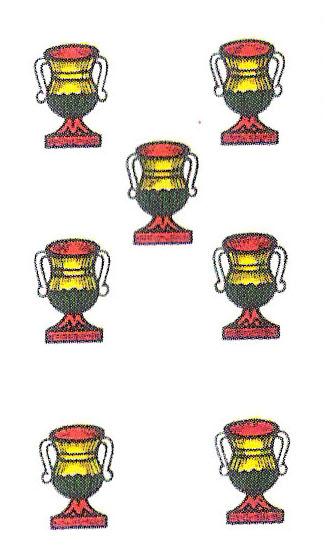
\includegraphics[width=.15\textwidth]{img/7C.jpg}
  \\[\smallskipamount]
  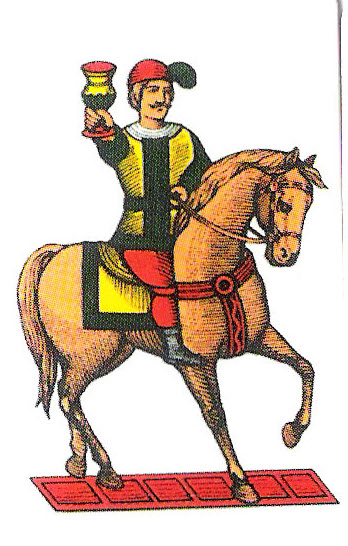
\includegraphics[width=.15\textwidth]{img/9C.jpg}\hfill
  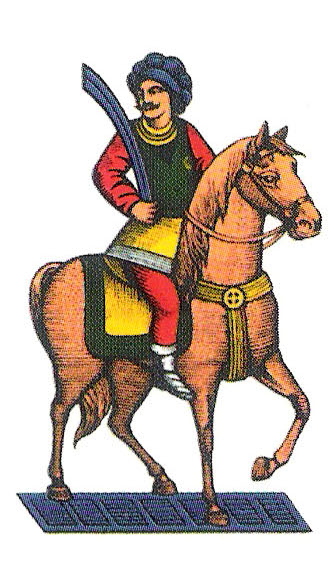
\includegraphics[width=.15\textwidth]{img/9S.jpg}
  \caption*{In order: a card with a special symbol, a basic suit card and 2 very similar cards}
\end{figure}

Color, in this case, serves as an invaluable supplementary feature, augmenting the existing shape properties to enhance classification accuracy.
In total we have to identify reliably 22 individual shapes considering:

\begin{itemize}
  \item the 8, 9 and 10 cards counted one time
  \item the basic suits to count
  \item the 4 "Assi" and other cards with special shapes like the 2 of swords
  \item other cards that have special symbols in them like the 5 of swords
\end{itemize}


\begin{figure}[H]
  
\includegraphics[width=.15\textwidth]{img/5S.jpg}\hfill
  
\includegraphics[width=.15\textwidth]{img/2S.jpg}
  \caption*{On the left a card with special symbols in it. On the right a unique card shape.}
\end{figure}


\subsection*{Experiment Platform}
The project is brought to life with the following equipment and software:
\begin{itemize}
  \item Pixel 6a with stock camera application for taking photos;
  \item Python 3.10.12 

\end{itemize}


\subsection*{Pipeline}
The Neapolitan Card Recognizer (NCR) project employs a pipeline that integrates image preprocessing, dataset generation with perspective transformations, feature extraction focusing on shape and color, and the use of machine learning for card classification. This structured approach ensures accurate recognition of Neapolitan playing cards from images, addressing challenges like image quality and variability through comprehensive preprocessing and leveraging a RandomForestClassifier for the identification of card types.
\begin{figure}[H]
  \centering
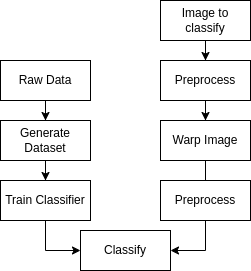
\includegraphics[width=.26\textwidth]{img/genralDescription.png}
\caption*{The pipeline used for the card capture and identification} 
\end{figure}


\subsection*{Card Capture}
The effectiveness of NCR hinges significantly on the robust detection of playing cards within a complex background. This section delves into the comprehensive methodology employed for card detection, detailing the steps from initial image acquisition to isolating potential card regions for further processing and classification.

\begin{figure}[H]
  \centering
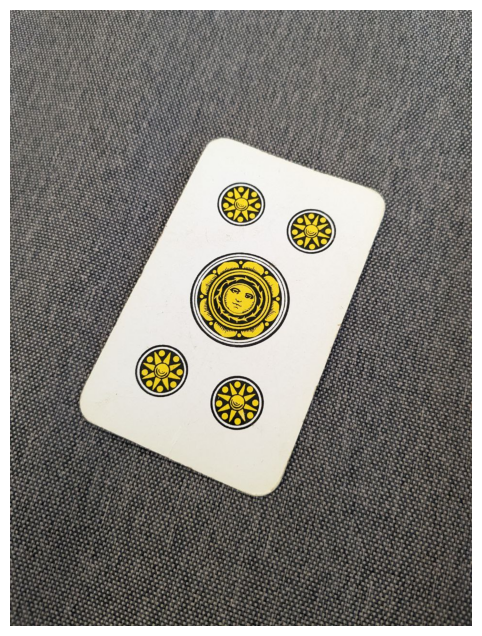
\includegraphics[width=.26\textwidth]{img/1-raw.png}
\caption*{Raw Image} 
\end{figure}

The journey begins with the acquisition of a high-definition image, which is then subjected to a series of preprocessing steps aimed at simplifying the detection process. Given the high resolution of images captured by the used camera, which can inadvertently emphasize minor imperfections on the card surface or background, an initial downsampling step is applied. This downsampling effectively reduces the image size by a factor of two, striking a balance between preserving essential details and minimizing unnecessary complexity.

We then apply a morphological operation to smooth the image morphology, creating a more uniform background and making it easier to isolate the card from the rest of the image. Specifically, a closing operation with a 3x3 kernel is employed, which is effective in reducing noise and small imperfections on the card and background.



\begin{figure}[H]
  \centering
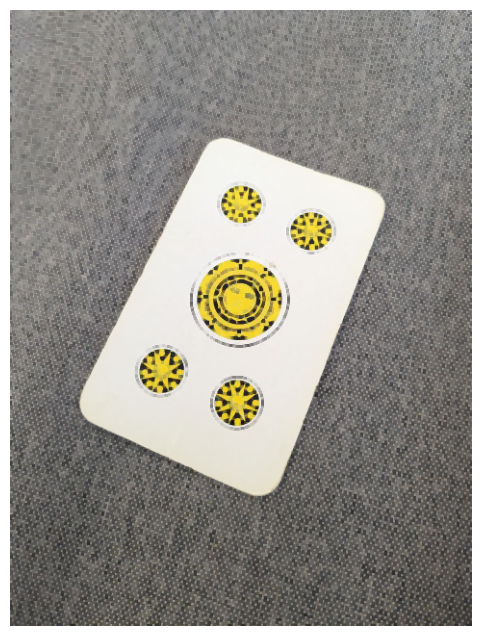
\includegraphics[width=.26\textwidth]{img/downsampled_and_morphed.png}
\caption*{Simplified image} 
\end{figure}


Following preprocessing, the image undergoes a binary conversion process. This critical step transforms the image into a binary format, starkly contrasting the card against its background, thereby facilitating the detection of its contours. For a more detailed explanation of the preprocessing refer to the dedicated subsection.

\begin{figure}[H]
  \centering
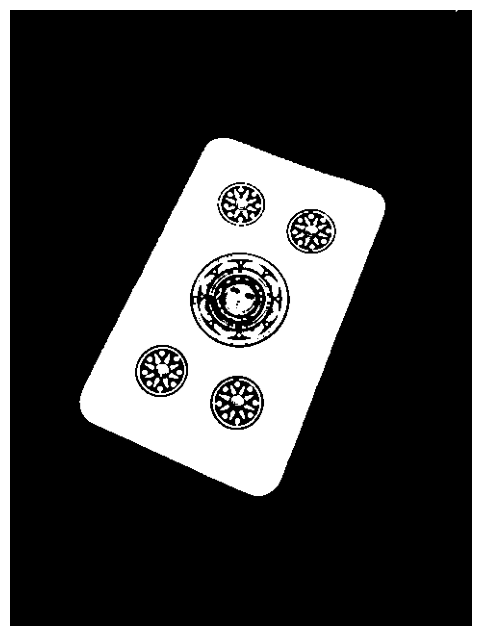
\includegraphics[width=.26\textwidth]{img/binary.png}
\caption*{Binarized Image} 
\end{figure}

To filter out insignificant contours, those too small to be cards, we order them based in a decrescent way based on the dimension of the area they take. The contours than are approximated using the \textbf{cv2.approxPolyDP}. The first contour with an area that is big enough in relation to the size of the image and has 4 corner is considered as the card to identify.

\begin{figure}[H]
  \centering
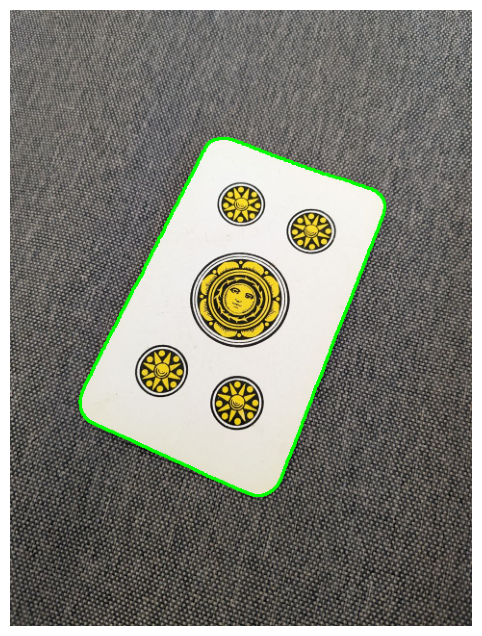
\includegraphics[width=.15\textwidth]{img/2-cardIdentified.png}\hfill
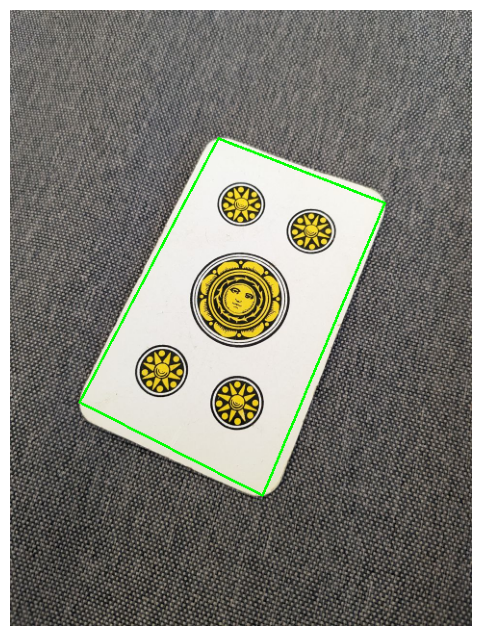
\includegraphics[width=.15\textwidth]{img/approx_card.png}\hfill
\caption*{Identified card Image and its approximated contour} 
\end{figure}

The corner points are than identified as the topLeft, topRight, bottomLeft and bottomRight corner supposing that the card is more or less in a vertical position in respect of the frame. This is done using the fact that the if we sum up the coordinates of the points, the topRight corner will have the minimum value and the bottom right the highest and if we differentiate the coordinates, the topRight will have the minimum value and the bottomRight the highest.

\begin{figure}[H]
  \centering
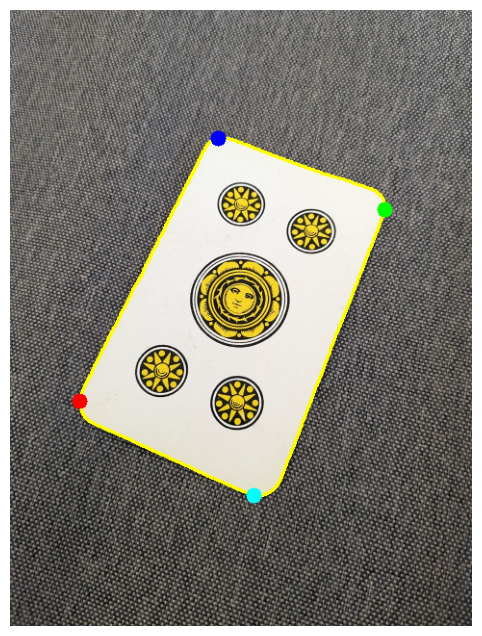
\includegraphics[width=.26\textwidth]{img/3-corner.png}
\caption*{Corners of the card} 
\end{figure}

These corners are than used to warp the prospective defining the new image dimensions using the maximum width between the top ans bottom corners and maximum height between the left a right corners. After that the new image will be generated using the \textbf{cv2.getPerspectiveTransform()} to get the warp matrix and the \textbf{cv2.warpPerspective()} with the new dimensions to obtain the end result.

\begin{figure}[H]
  \centering
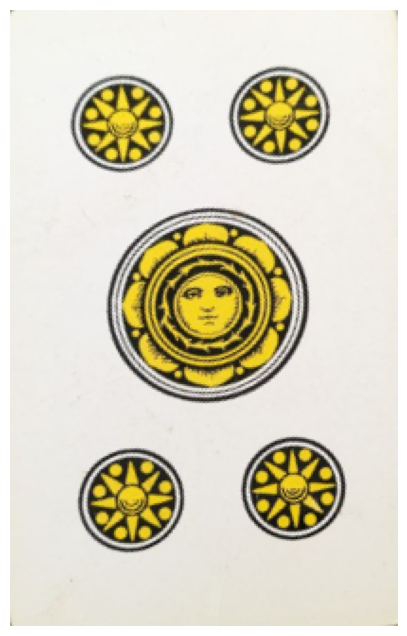
\includegraphics[width=.26\textwidth]{img/4-warped.png}
\caption*{Warped card} 
\end{figure}

\subsection*{Preprocessing}

Preprocessing serves as a critical foundation for the subsequent detection and recognition of Neapolitan cards. This stage involves several key procedures designed to enhance the image quality and isolate features crucial for accurate classification. The comprehensive preprocessing pipeline includes  white balance correction, grayscale conversion, median blurring, image inversion and contrast enhancement, and contour extraction. Each step is tailored to address specific challenges presented by the raw images and is crucial for the robust performance of the NCR.
 
\begin{figure}[H]
  \centering
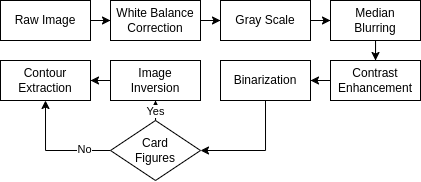
\includegraphics[width=.4\textwidth]{img/Preprocessing-Pipeline.png}
\caption*{The pipeline used for the card capture and identification} 
\end{figure}

\subsubsection*{White Balance Correction}
Given the variability of lighting conditions under which the images might be captured, the inconsistencies given by the auto white balance of the camera app, a white balance correction step is applied to ensure color consistency across different images. This step adjusts the image's color temperature, making the colors appear more natural and consistent, which is crucial for accurate feature extraction and classification later in the process.

The correction process involves converting the image to a floating-point representation to compute the average value for each color channel (blue, green, and red). Scaling factors are then calculated to adjust each channel's average to match the overall average brightness, effectively neutralizing color casts caused by different lighting conditions.
\begin{figure}[H]
  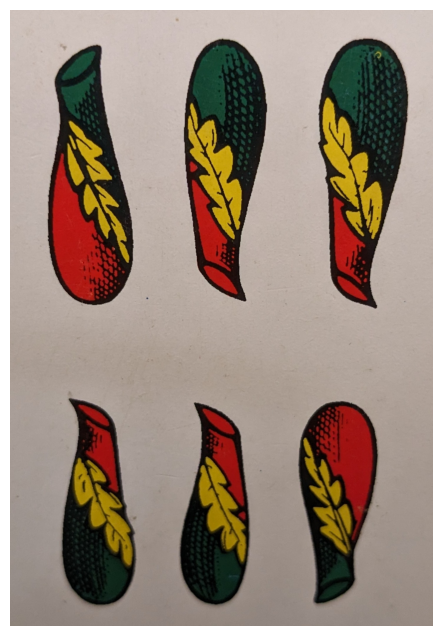
\includegraphics[width=.23\textwidth]{img/w1.png}\hfill
  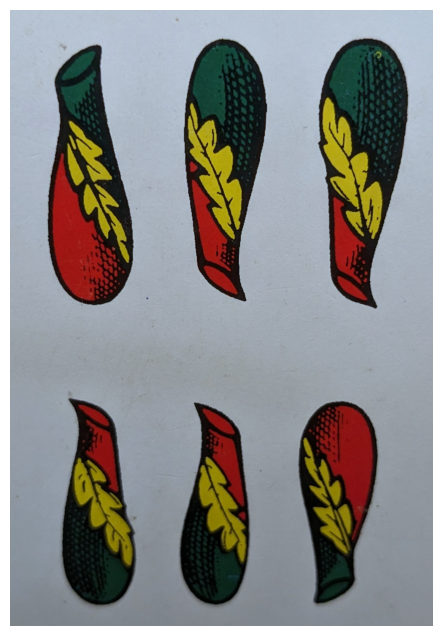
\includegraphics[width=.23\textwidth]{img/w2.png}

  \caption*{Card before and after white balance}
\end{figure}

\subsubsection*{Grayscale Conversion and Median Blurring}

To simplify the detection of contours and reduce the computational complexity, the image is converted to grayscale using the \textbf{cv2.cvtColor} function. This conversion discards color information, focusing on intensity variations (in 256 levels) that are essential for identifying card shapes and features.

Following grayscale conversion, a median blur is applied to the image using \textbf{cv2.medianBlur} function with a 3x3 kernel. This type of blurring is effective in reducing noise and minor imperfections, such as dust specks, without significantly blurring the edges of the card. It helps in cleaning the image while avoiding an heavy impact on the contours of the image, without using edge preserving filters that could hinder performance. This is important especially during the ingestion of the massive dataset.

\subsubsection*{Contrast Enhancement}
After median blurring, the image undergoes a contrast enhancement step. This is achieved by adjusting the image's contrast and brightness levels, making the card's features more pronounced and easier to detect. It is done using the \textbf{cv2.convertScaleAbs} function. Enhanced contrast is particularly beneficial for highlighting the edges and details of the cards, which are critical for accurate identification.

\subsubsection*{Binarization}
Once we have gotten the best card image possible we can binarize the image (convert each pixel in a 1 or 0). Taking in consideration that we are working with cards that a this point have pretty uniform background and a high contrast we can use a high treshold to set pixels to 1. We use the \textbf{cv2.threshold}  with a treshold of 155.

\subsubsection*{Image Inversion and Contour Extraction}
For the contour extraction we have to distinguish between when we have photos of black subjects on white backgrounds(identify card shapes on the white of the cards background) and the inverse(mostly white cards on a dark background).

Since the contour extraction function \textbf{cv2.findContours} works in the second case, we have to implement a function to invert the binary values from the binarization when identifying the figures on the card.

This process involves identifying continuous curves that delineate the card's boundaries from the rest of the image. Contours are detected by applying edge detection algorithms to the preprocessed image, followed by the retrieval of outlines that represent potential card shapes.

The contours are then sorted and possibly filtered based on their area to ensure that only relevant contours, likely to represent cards or cards figures, are considered in the subsequent processing stages. This selective approach streamlines the recognition process, focusing computational resources on the most promising candidates.
\\
\subsection*{Dataset}
The creation of a robust and varied dataset is pivotal for the development of any machine learning system, including the Neapolitan Card Recognizer (NCR). This section outlines the methodology adopted for generating a comprehensive dataset of Neapolitan cards, focusing on the techniques employed to simulate a wide range of real-world conditions under which the cards might be photographed.

\subsubsection{Initial Setup and Preprocessing}
The dataset generation process begins with a collection of high-quality digital scans of Neapolitan cards. These scans are manually cropped to isolate individual cards, ensuring clarity and consistency across the initial dataset. To create a more resilient classifier is than applied a perspective transformation. 

\subsubsection{Perspective Transformation}
A crucial step in dataset augmentation is the application of perspective transformations to the card images. This process simulates the effect of capturing photos from various angles and distances, introducing realistic distortions akin to those seen in everyday use. Is than applied a random perspective change.

The objective is to generate a unique perspective matrix for each image based on random parameters. The parameters for the matrix are determined using a combination of fixed seeds for repeatability and random number generation to introduce controlled randomness into the transformation process.
\begin{equation}
  \centering
  \begin{bmatrix}
    1+r & 0+r & 0+r\\
    0+r & 1+r & 0+r\\
    0 & 0 & 1+r
  \end{bmatrix}
\end{equation}
\captionof{mat}{Perspective matrix applied for the transformation. The value "r" is random value between -0.02 and 0.02 that is different for each element of the matrix}

To accommodate the distortions without clipping the card images, each card is first placed centrally within a larger canvas before the perspective transformation. This step ensures that the entirety of the card remains visible post-transformation, regardless of the distortion applied.

Each card image undergoes the random perspective change a predetermined number of times (in this case, 24 iterations per card). This process results in a significantly augmented dataset, with each original image yielding 24 uniquely transformed variants. These variants are saved to a new dataset directory, systematically labeled to facilitate easy identification and retrieval.
\begin{figure}[H]
    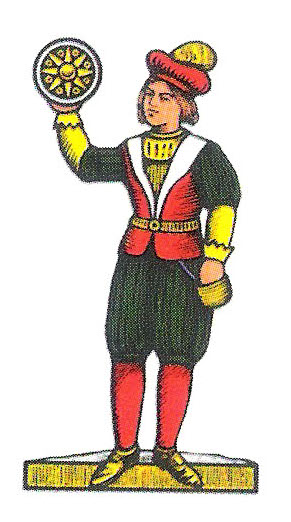
\includegraphics[width=.15\textwidth]{img/w_cards/w_card1.jpg}\hfill
    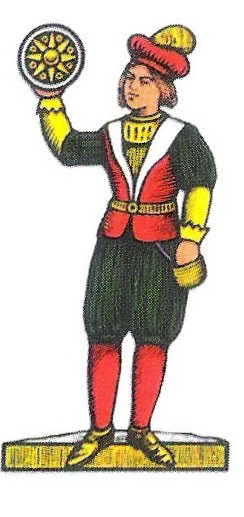
\includegraphics[width=.15\textwidth]{img/w_cards/w_card2.jpg}
    \\[\smallskipamount]
    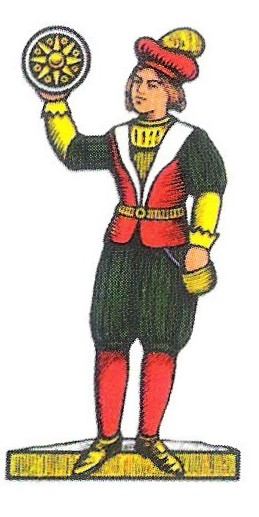
\includegraphics[width=.15\textwidth]{img/w_cards/w_card3.jpg}\hfill
    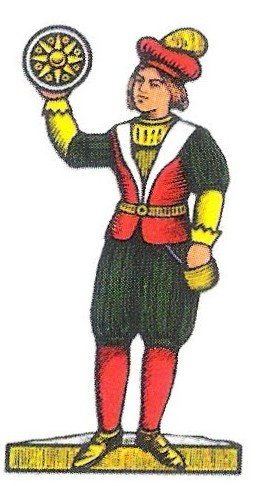
\includegraphics[width=.15\textwidth]{img/w_cards/w_card4.jpg}
    \caption*{Original card and 3 warped versions}
\end{figure}

The labels incorporate both the card's characteristics (value, seed) and the iteration of the transformation, allowing for precise tracking of data provenance and characteristics.

Each processed image, complete with detected contours, is saved back to the working directory, to have the possibility to manually check the effectiveness of the generation.

\subsection*{Classification}

The classification stage is the culmination of the Neapolitan Card Recognizer (NCR) process, where the system leverages machine learning algorithms to accurately identify the type of card present in an image. This section details the methodology employed in the card classification process, highlighting the data preparation, feature extraction, model training, evaluation, and the utilization of the classification model for predicting card types.

\subsubsection*{Data Preparation and Feature Extraction}
The classification process begins with the preparation of a dataset comprising images of Neapolitan cards that have been subjected to perspective transformations to simulate real-world conditions. Each image in the dataset is processed to extract two main types of features: Hu Moments and the average hue. Hu Moments are used to capture the shape information of the cards, while the average hue captures the color information, both of which are crucial for distinguishing between different types of Neapolitan cards.

Hu Moments: These moments are calculated for each card's biggest contour, providing a seven-element feature vector that describes the shape of the card. These features are scale and rotation invariant, useful not only for part of the perspective alteration not corrected by the card capture step, but for identification of the rotated shapes of the basic suits.  These moments were calculated using the function \textbf{cv2.HuMoments} applied on the moments obtained with \textbf{cv2.moments}.

\begin{figure}[H]
  \centering
  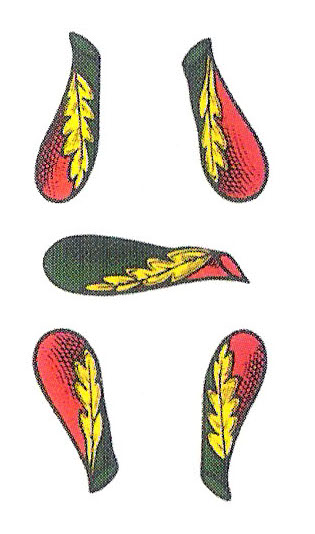
\includegraphics[width=.23\textwidth]{img/5B.jpg}

  \caption*{Card with the same basic contour repeated and rotated}
\end{figure}

Average Hue: This feature represents the average color hue within the contour of the card, adding an additional dimension to the feature set. This value is obtained averaging the hue value obtained in the pixels inside the contour after that the image was brought to the HSV color space.
This conversion was used to obtain a single value to consider for color to avoid adding too many features to classify from.

All of these features are than concatenated to form a comprehensive feature vector for each card, which serves as the input for the machine learning model.

\subsubsection*{Model Training}
For the classification model, a RandomForestClassifier from the scikit-learn library is chosen due to its effectiveness in handling non-linear data and its ability to model the complex relationships between the shape and color features of the cards. The dataset is split into training and testing subsets to evaluate the model's performance accurately. A StandardScaler is applied to the feature vectors to normalize the data, ensuring that the model is not biased by the scale of the features.

The RandomForest model is trained on the normalized training data, with the label for each image indicating the type of Neapolitan card (e.g., "RO" for "Re" of "Oro"). For the cards with basic suits to count, the label is only the suit type: B for "Bastoni", S for "Spade", O for "Oro" and C for "Coppe". The number of estimators for the RandomForestClassifier is set to 10, providing a balance between model complexity and performance.

\subsubsection*{Evaluation and Prediction}
After training, the model's accuracy is evaluated on the testing subset of the dataset. The accuracy score and a detailed classification report provide insight into the model's performance across different card types. Additionally, a confusion matrix is generated to visualize the model's predictions compared to the true labels, highlighting areas where the model may be confusing one card type for another \ref{fig:c_matrix}.

\begin{figure}
  \centering
  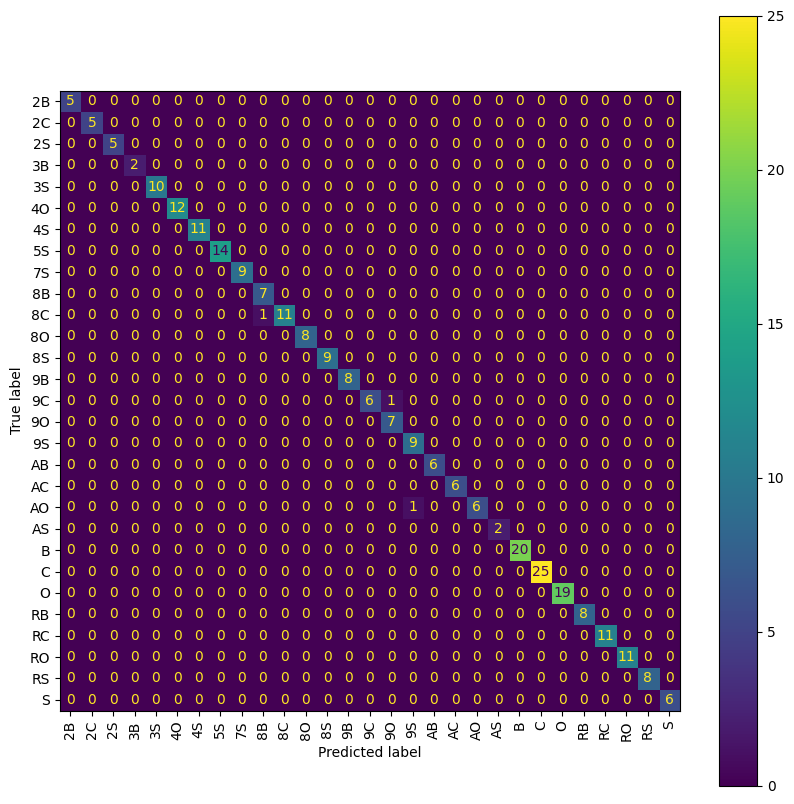
\includegraphics[scale=0.4]{img/confusionMatrix.png}
  \caption{Confusion Matrix that represent accuracy using the generated dataset. The contours to count are labeled as basic Suits [B,C,O,S]}
  \label{fig:c_matrix}
\end{figure}

For cards that falls in the category of simple shapes to count (for example the 7 of "Bastoni") we can predict the other "smaller" contours and see if they are of the same type.

The trained RandomForest model, along with the scaler, is then saved to disk for future use in classifying new card images.

\section*{Conclusion and Future Developments}

The Neapolitan Card Recognizer project represents a study advancement in the application of machine learning and computer vision techniques to the identification and classification of traditional playing cards. Through meticulous preprocessing, robust dataset generation, and sophisticated classification methodologies, the NCR demonstrates high accuracy in recognizing Neapolitan cards under a variety of conditions. This system not only serves as a valuable tool that showcases the potential for applying similar technologies to other areas of cultural heritage and digital humanities.

\subsection*{Achievements}
The development of the NCR system highlighted several key achievements:
\begin{itemize}
  \item The creation of a versatile preprocessing pipeline that enhances image quality and isolates critical features for card recognition.
  \item The creation of a pipeline that can be easily adapted for different card games.
  \item The generation of a comprehensive and varied dataset of card images, simulating real-world conditions through perspective transformations.
  \item The implementation of a robust classification model capable of distinguishing between different types of Neapolitan cards with high accuracy.
\end{itemize}



\subsection*{Future Developments}
While the current iteration of the NCR has proven effective, there are several avenues for future development that could enhance the system's performance and usability:

\begin{itemize}
  
  \item \textbf{Simplification of the Identification Process:} One of the potential improvements involves simplifying the card identification process by reducing or eliminating the need for warping images during identification. This could involve developing more advanced algorithms capable of recognizing cards from various angles and conditions without the need for extensive preprocessing. Such a simplification could significantly speed up the recognition process and reduce computational requirements.

  \item \textbf{Expansion of the Dataset:} Expanding the dataset to include a wider range of card designs, conditions, and backgrounds could further improve the model's robustness and accuracy. Incorporating user-generated content and leveraging crowdsourcing platforms could provide a cost-effective way to enrich the dataset.

  \item \textbf{User Interface Development:} Developing a user-friendly interface for both dataset augmentation and card recognition could make the NCR more accessible to a broader audience, including researchers, game developers, and enthusiasts. This could facilitate the adoption of the NCR in practical applications for the use with the visually impaired people.

  \item \textbf{Real-time Recognition:} Implementing real-time card recognition capabilities could open up new possibilities for interactive applications, such as augmented reality games or educational tools that provide instant feedback or information about the cards.

  \subsection*{Conclusion}   
The Neapolitan Card Recognizer project stands as a testament to the power of combining traditional cultural elements with cutting-edge technology. As we look to the future, the potential for further development and application of the NCR is vast, promising not only to enhance our understanding and appreciation of Neapolitan cards but also to pave the way for innovative applications of machine learning and computer vision in cultural preservation and beyond.
\end{itemize}
\nocite{*}
\bibliographystyle{BSO2022}
\bibliography{references}
\newpage
\onecolumn
\end{document}
